%\documentclass[leqno,11pt]{jarticle}
\documentclass [dvipdfmx] {jsarticle}
%\documentclass[a5j]{jarticle}

\makeatletter
\RequirePackage{marginnote,xcolor}
\setlength{\marginparsep}{5pt}
\let\temp@label\label
%\def\label#1{\marginnote{\hbox to 0pt{\scriptsize \textcolor{black!60}{#1}\hss}}\temp@label{#1}\ignorespaces}
\makeatother
\usepackage[mathscr]{eucal}
\usepackage{mathrsfs}
\usepackage{amscd}
\usepackage{amsfonts}
\usepackage{amsmath, amsthm, amssymb}
\usepackage{latexsym}
\usepackage{bm}
\usepackage[dvips]{graphics}
\usepackage{color,graphicx}
\usepackage{pdfpages}
\usepackage{algorithmic}
\usepackage{algorithm}


\numberwithin{equation}{section}

\def\tr#1{\mathord{\mathopen{{\vphantom{#1}}^t}#1}} 
\def\C{{\mathbf{C}}}%   \C == \mathbf{C}
\def\R{{\mathbf{R}}}%   \R == \mathbf{R}
\def\Q{{\mathbf{Q}}}%   \Q == \mathbf{Q}
\def\H{{\mathbf{H}}}%   \H == \mathbf{H}
\def\Z{{\mathbf{Z}}}%   \Z == \mathbf{Z}
\def\N{{\mathbf{N}}}%   \N == \mathbf{N}
\def\A{{\mathcal{A}}}%  \A == \mathcal{A}
\def\D{{\mathbf{D}}}%  \D == \mathbf{D}
\def\L{{\mathbf{L}}}%  \L == \mathbf{L}
\def\W{{\mathcal{W}}}% \W == \mathcal{W}
\def\Pa{{\mathbf{P}}}%  \Pi == \mathbf{P}
\def\Si{{\mathbf{S}}}%   \Si == \mathbf{S}

\theoremstyle{definition} %
\newtheorem{theorem}{\bf 定理}[section] % 
\newtheorem{lemma}[theorem]{\bf 補題}
\newtheorem{corollary}[theorem]{\bf 系}
\newtheorem{proposition}[theorem]{\bf 命題}
\newtheorem{fact}[theorem]{\bf 事実}
\newtheorem{conjecture}[theorem]{\bf 予想}
%
\theoremstyle{definition} % 
\newtheorem{definition}[theorem]{\bf 定義}
\newtheorem{remark}[theorem]{\bf 注意}
\newtheorem{example}[theorem]{\bf 例}
\newtheorem{notation}[theorem]{\bf 記号}
\newtheorem{assertion}[theorem]{\bf 要請}

\renewcommand{\proofname}{\bf 証明.}
\renewcommand{\algorithmicrequire}{\textbf{Input:}}
\renewcommand{\algorithmicensure}{\textbf{Output:}}


\pagestyle{plain} 

\title{Master Thesis \\ \bigskip 
修士論文 \\ \bigskip 
{\bf  遅延微分方程式を用いたプレス機制御法の開発 }\\ \bigskip 
} 
\author{九澤俊介}
\date{金沢大学大学院自然科学研究科 \\
Graduate School of Natural Science and Technology, \\
Kanazawa University}

\begin{document}
\maketitle
\thispagestyle{empty}
\setcounter{page}{-1}


\thispagestyle{empty}

\mbox{}\newpage 

\tableofcontents
\clearpage
\section{はじめに}
遅延微分方程式とは,現時点の時間導関数が解だけでなく,前の時間における導関数にも依存する可能性のあるような微分方程式である.
制御システムにおいてフィードバックにかかる時間遅れも指摘されており,様々な数理モデルが数多く研究されている.
身近な例としては,シャワーの温度調節が上げられる.熱いと感じて温度を下げるがぬるすぎて再び温度を上げるなどのような
ことが挙げられる.\\
また本研究は,東和精機株式会社と共同研究である.同社の制御システムに遅延微分方程式を応用した.
\subsection{目的}
本研究では遅延微分方程式で数理モデルを構築し,株式会社東和精機のプレス制御法の開発を行う.
東和精機では,車のタイヤの連結部分であるシャフトをプレスすることによりその形状を成型している.
その際に,プレス機の制御システムにおいてフィードバックに時間がかかることで時間遅れが生じる.
そして時間遅れが生じることで,目的のプレスしたい量と実際にプレスした量が一致しない問題があった.
そこでこのプレス制御に対して時間遅れ微分方程式で数理モデルを構築することで,目的のプレスしたい量と実際にプレスした量が一致させる
方法を開発するために本研究に至った.
(プレス機のイメージ図)


\subsection{本論文の構成}
本論文は次のように構成される.第2節では東和精機の問題の具体的な概要、また本論文で扱う記号などについて述べる.
第3節では$\beta$コントロールによるプレス制御モデルと
そのモデルによる数値シミュレーションの結果を表す.
第4節では線形コントロールによるプレス制御モデルとそのモデルによる数値シミュレーション
結果を表す.第5節では第4節のモデルで得られた結果から見える今後の課題や展望などについて述べる.


\section{概要}
金属棒の歪んでいる方向と反対側へ指定の位置までプレスすることに
よって,真っ直ぐの状態に塑性変形させ金属棒の歪みをとりたいのだが,
現実にはその指定位置を超えてプレスしてしまう現象 (オーバーシュート) が起こる.
オーバーシュートが生じる原因として,計測結果が歪取機に反映されるまでの遅れが挙げられる.
時間遅れは東和精機に計測していただいたデータを用いる.
\begin{figure}[hbt]
    \centering
    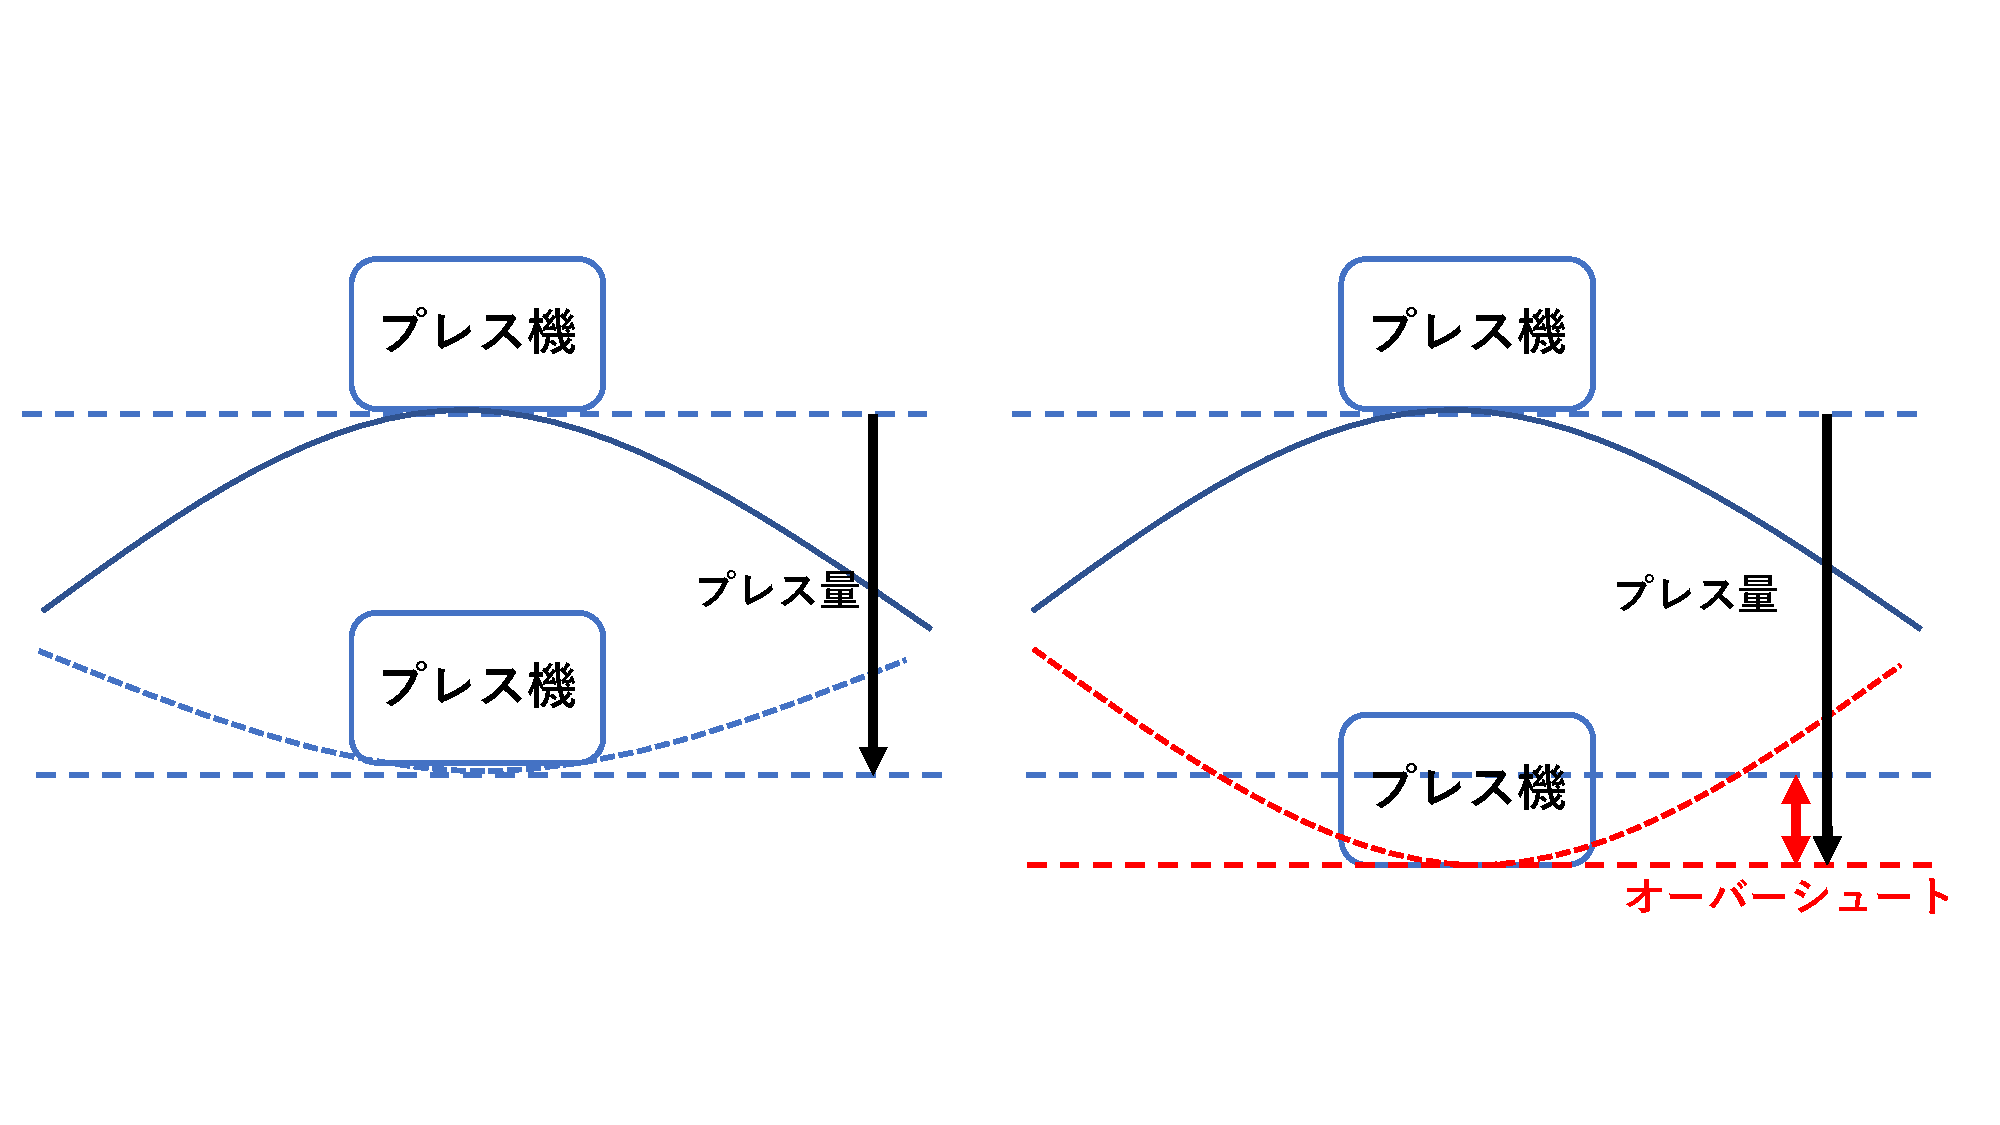
\includegraphics[scale=0.5,keepaspectratio]{/Users/shunsuke/Desktop/master-thesis/press_image.pdf}
    \caption{理想の状態(左)と実際の状態(右).}
    \label{Sample p.1}
\end{figure}
\newpage
%%\includepdf[noautoscale=true, scale=0.9, pagecommand={}]{修論図_2.pdf}


\section{$\beta$コントロールによる分析}
\subsection{制御モデルについて}
次のプレス制御を考える.
ただし,シャフトをプレス機で押し込みたい量を$\ell$,制御システムにおいて発生する時間遅れを$\tau$,プレス速度の最大値を
$v_{\max}$,最小速度を$v_{\min}$,時刻$t$において得られる最新の位置情報を$X(t)(=x(t-\tau))$とする.
\begin{equation}\label{eq:betamodel}
    V(X)=v_0\left(\frac{\ell-X}{\ell}\right)^\beta.
\end{equation}
\\ただし,$X(t)=0\ \ (0\le t\le\tau)$とする.
\\
この制御方法は,プレス機の位置が目標のプレス量に近づくにつれて減速していく.それはプレス機が時間遅れのためすぐに停止できず
オーバーシュートしてしまうため,プレス機の位置が目標のプレス量に十分近い時,低速である必要があるからである.\\
この制御方法に対して,与えられた$\ell,\tau,\beta$に対して,オーバーシュートが生じず、プレス時間が最も短く済む
ような,初速$v_0$を求める.

% \begin{equation}
%     V(X)=v_0\left(\displaystyle\frac{\min\{\ell_1,\ell-X\}}{\min\{\ell_1,\ell\}}\right)^\beta.
% \end{equation}
% $X$が十分に$\ell$に近づけば停止させる.



% 指数$\beta$に対し,
% \begin{equation}
%     G:=1-0.58\times\beta^{-0.79},\ \ell_1:=\frac{\tau v_{\max}}{G},\ v_0:=\min\left\{\displaystyle\frac{\ell G}{\tau},v_{\max}\right\}
% \end{equation}
% とおく.次のようにプレス速度$V(X)$を設定する.


\subsection{微分方程式}
$t\in\mathbb{R},x(t)\colon\mathbb{R}\rightarrow\mathbb{R}$と定数$\ell,\tau$,
上で定めた$\beta,v_0$に対して\eqref{eq:betamodel}は次のように書き換えられる.
\begin{equation}\label{betafomula}\begin{cases}
    \displaystyle\frac{dx}{dt}(t)=v_0\left(\frac{\ell-x(t-\tau)}{\ell}\right)^\beta &(t>\tau),\\
    x(t)=v_0 t &(0\le t \le \tau).
\end{cases}\end{equation}


\subsubsection{無次元化}
次のような記号を用いると
\begin{equation}
    s:=\frac{t}{\tau},\ w(s):=\frac{x(\tau s)}{\ell},\ u_0:=\frac{\tau v_0}{\ell},
\end{equation}
\eqref{betafomula}は次のように書ける.
\begin{equation}\label{betafomula2}\begin{cases}
    \displaystyle\frac{dw}{ds}(s)=u_0(1-w(s-1))^\beta &(s>1),\\
    w(s)=u_0 s &(0\le s \le 1).
\end{cases}\end{equation}


\subsection{数値計算}
\subsubsection{離散化}
$2\le K\in\mathbb{N}$として,時間刻み幅を$\Delta t:=\frac{1}{K}$とおく.
初期条件を$W_n=u_0n\Delta t (n=0,1,...,K)$として,$w_n $ ($n=K+1,K+2,...$)
を次で求める.
\begin{equation}
    \displaystyle\frac{w_{n+1}-w_n}{\Delta t}=u_0(1-w_{n-K})^\beta.
\end{equation}
\subsubsection{アルゴリズム}
\begin{figure}[h]
    \begin{algorithm}[H]
        \caption{Calculate $\beta$コントロール}
        \label{alg1}
        \begin{algorithmic}[1]    
        \REQUIRE $2\le K \textless N\in\mathbb{N}$
        \ENSURE $y = x^n$
        \FOR{$n \le N$}
        \IF{$n \le K$}
        \STATE $y \leftarrow 0$
        \ELSE
        \STATE $y \leftarrow X[n-K]$
        \ENDIF
        \STATE $X[n+1]\leftarrow X[n]+\left(\displaystyle\frac{\min(|L-y|,L1)}{L_{\min}}\right)\times v\times dt$
        \ENDFOR
        \end{algorithmic}
    \end{algorithm}
\end{figure}
\subsubsection{数値計算結果}
($\beta$を固定して$u_0$をパラメータとした結果)
\section{線形コントロールによる分析}
従来の$\beta$コントロールでは以下のような課題があった.
\begin{itemize}
    \item プレス機をシャフトに衝突してから制御し始めていたため,押込量が小さいときオーバーシュートが大きくなる.
    \item 初速を$v_0(<v_{\max})$にすると,時間がかかる.
    \item 停止直前の速度が小さすぎる.
    \item 制御速度が押込量に依存しているため,オーバーシュートが安定しない.
\end{itemize}
このような課題を受け,以下のような改善点を基に線形モデルを構築した.
\begin{itemize}
    \item \eqref{betafomula}について$\beta=1$として線形コントロールすることでプレス機の速度を上げる. 
    \item 初速は常に$v_{\max}$とする.
    \item 押込量が小さいときはプレス機がシャフトに接触する前から制御を始める.
    \item 制御速度を押込量に依存させないようにする.
\end{itemize}
\eqref{betafomula}について$\beta=1$とすると,プレス速度が上がり,オーバーシュートが大きくなってしまうという問題が発生してしまう.そのため考案したアイデアが
目的のプレスしたい量の手前でプレス機を止める指令を出すことである.目的のプレスしたい量$\ell$に対して,少し手前で止める量$\ell_0$を
以下のように定義する.
\begin{equation}\label{delta_ell}
    \Delta\ell :=\delta v_{\min}\tau,\ \ell_0:=\ell-\Delta\ell
\end{equation}
ただし,$\delta$はパラメータ,$v_{\min}$は最小速度,$\tau$は時間遅れである.
目標のプレスしたい量$\ell$から$\Delta\ell$手前で止め,最小速度で時間遅れ分プレスされ,目標のプレスしたい量で止まる
という考えである.\\
また,$\beta$コントロールではプレス機をシャフトに衝突してから制御していたが,線形コントロールでは,シャフトに衝突する前に制御を開始する.\\
$\beta$コントロールでは制御開始点$x(0)=0$としていたが,線形コントロールでは,
\begin{equation}\label{x_star}
    x_\ast:=\ell_0-\displaystyle\frac{v_{\max}-v_{\min}}{\alpha}\tau
\end{equation}
と定義し,制御開始点を$x(0)=x_\ast$と設定する.\\
$x_\ast$を設定することで,
押込量が小さい場合,プレス機がシャフトに衝突する前に制御を始めることが可能になる.
したがって線形コントロールでは\eqref{delta_ell}\eqref{x_star}で定義した$\Delta\ell , x_\ast$を用いて制御する.

\begin{figure}[hbt]
    \centering
    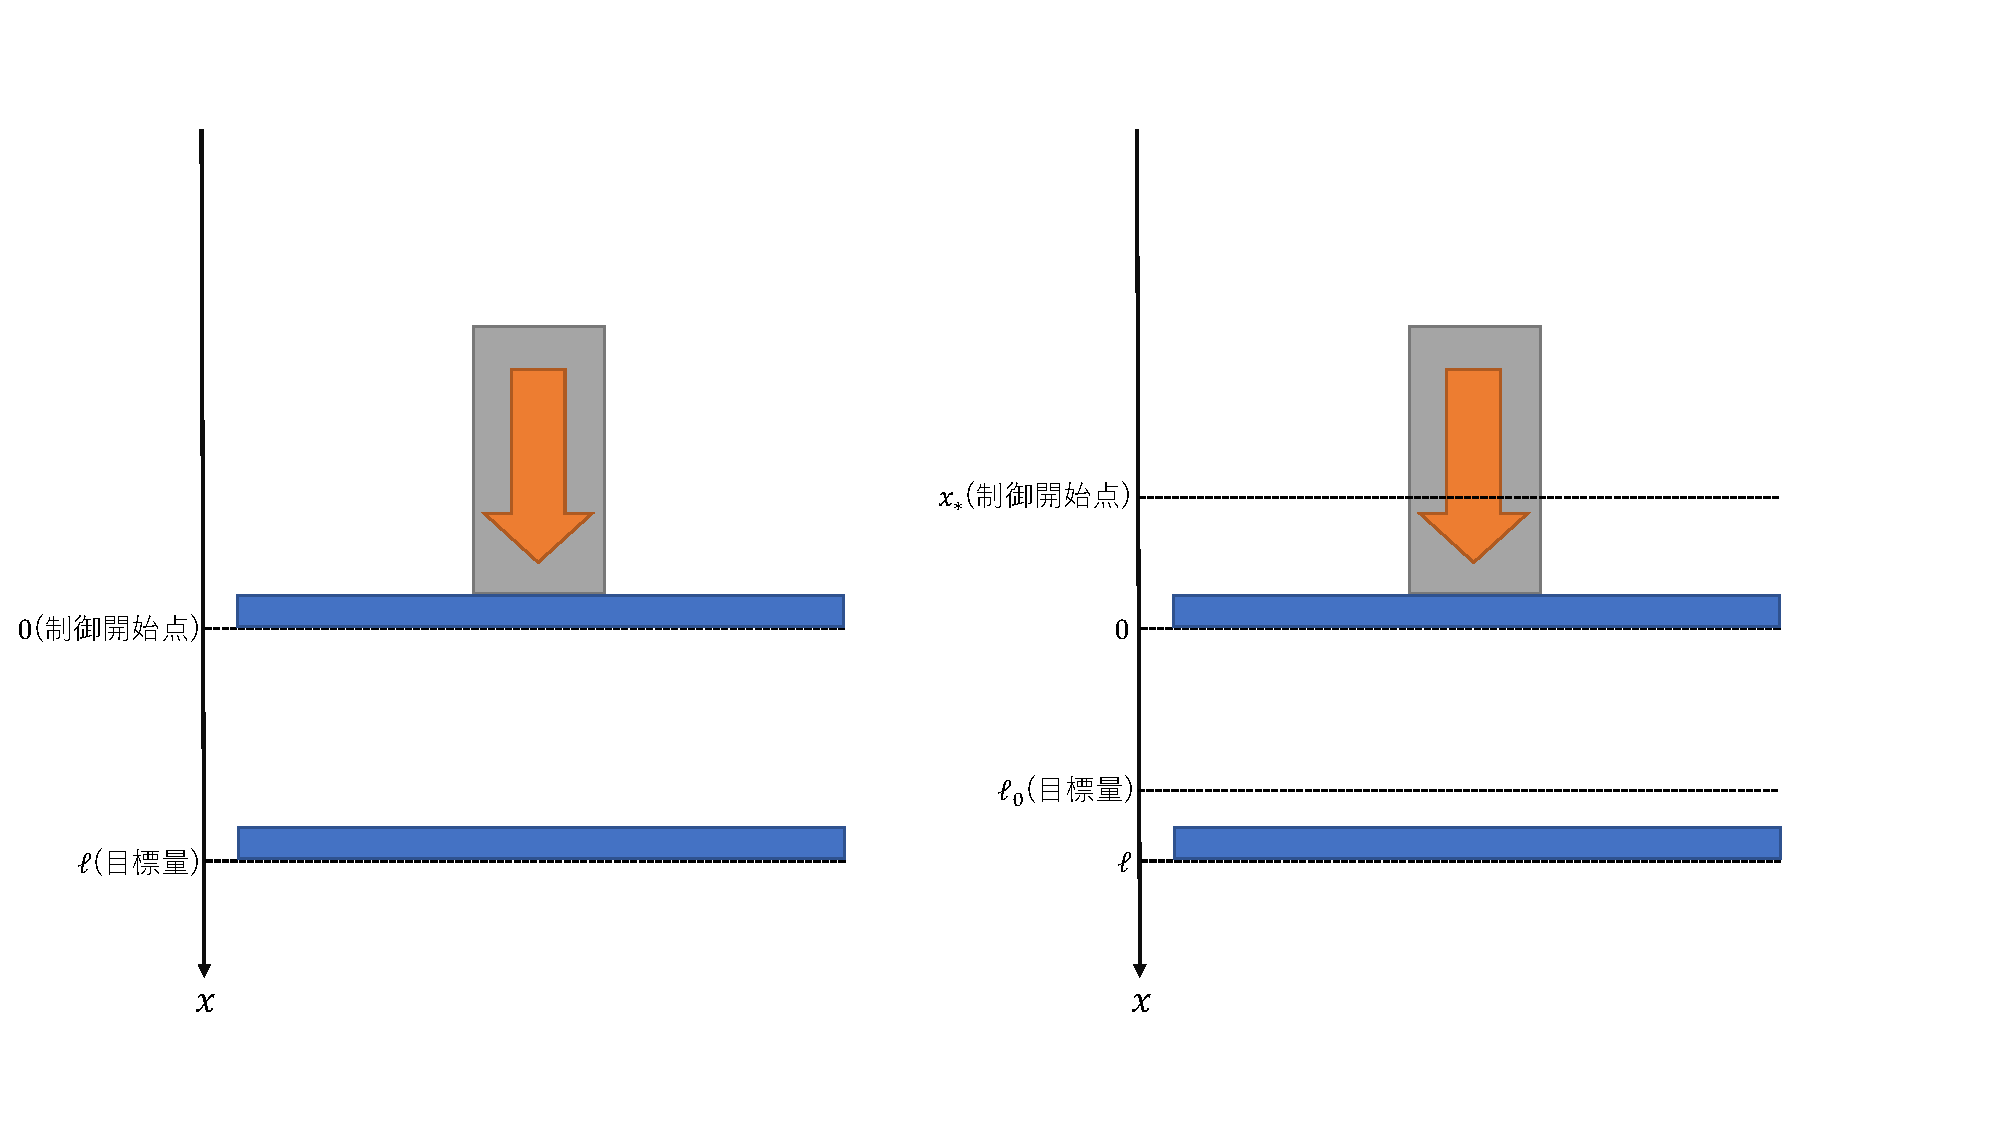
\includegraphics[scale=0.5,keepaspectratio]{/Users/shunsuke/Desktop/master-thesis/press_exp.pdf}
    \caption{$\beta$コントロール(左)と線形コントロール(右).}
    \label{Sample p.2}
\end{figure}
\subsection{制御モデルについて}
$\ell:$目標のプレスする距離,\ $\tau:$時間遅れ,\ $\alpha,\delta:$パラメータ,\ 
$v_{\max}:$プレス速度の最大値,\ $v_{\min}:$プレス速度の最小値,\ $X(t):$
時刻$t$で得られる最新の位置情報$(=x(t-\tau))$に対し,
\begin{equation}
    \Delta\ell :=\delta v_{\min}\tau,\ \ell_0:=\ell-\Delta\ell,\ a:=\frac{\alpha}{\tau}
\end{equation}
とし,$V(X)$を次のように設定する.
\begin{equation}\label{eq:linermodel}
    V(X)=v_{\min}+a(\ell_0-X)
\end{equation}
$X$が$\ell_0$に十分近づけば停止させる.


\subsubsection{微分方程式}
\eqref{eq:linermodel}は次のように書き換えられる.
\begin{equation}\label{eq:liner}\begin{cases}
    \displaystyle\frac{dx}{dt}(t)=v_{\min}+a(\ell_0-x(t-\tau)) &(t>\tau),\\
    x(t)=v_{\max}t+x_\ast &(0\le t \le \tau)
\end{cases}\end{equation}
ただし,$x_\ast$は\eqref{x_star}で定義した位置.

\subsubsection{正規化}
次のような記号を用いると
\begin{equation}
    s:=\displaystyle\frac{t}{\tau},\ y(s):=\displaystyle\frac{x(\tau s)}{v_{min}\tau},\
    d_0:=\frac{\ell_0}{v_{\min}\tau},\ u_{\max}:=\displaystyle\frac{v_{\max}}{v_{\min}},\ 
    y_\ast:=d_0-\displaystyle\frac{(u_{\max}-1)}{\alpha}
\end{equation}
\eqref{eq:liner}は次のように書ける.
\begin{equation}\label{eq:liner2}\begin{cases}
    \displaystyle\frac{dy}{ds}(s)=1+\alpha(d_0-y(s-1)) &(s>1),\\
    y(s)=u_{\max}s+y_\ast &(0\le s \le 1).
\end{cases}\end{equation}
さらに$z(s):=d_0-y(s)$とおくと,\eqref{eq:liner2}は次のように書ける.
\begin{equation}\label{z_press}\begin{cases}
    \displaystyle\frac{dz}{ds}(s)=1-\alpha z(s-1) &(1\le s\le s_\ast),\\
    z(s)=\displaystyle\frac{1}{\alpha}(u_{\max}-1)-u_{\max}s &(0\le s\le 1).
\end{cases}\end{equation}
$z(s)$が$0$に十分近づけば停止させる.
\eqref{z_press}は$\alpha,\ u_{\max}$に依存しており,$u_{\max}$は機械によって決まっている.\\
したがって,最適なプレス制御となるパラメータ$\alpha$を数値計算により決定する.


\subsection{数値計算}


\subsubsection{離散化}
$2\le K\in\mathbb{N}$として,時間刻み幅を$\Delta t:=\frac{1}{K}$とおく.
初期条件を$z_n=\frac{1}{\alpha} (u_{\max}-1)-u_{\max} n \Delta t$ ($n=0,1,...,K$)として,$w_n$ ($n=K+1,K+2,...$)
を次で求める.
\begin{equation}\label{z_method}
    \displaystyle\frac{z_{n+1}-z_n}{\Delta t}=1-\alpha z_{n-K}
\end{equation}
\subsubsection{アルゴリズム}
\begin{figure}[h]
    \begin{algorithm}[H]
        \caption{Calculate $\beta$コントロール}
        \label{alg1}
        \begin{algorithmic}[1]    
        \REQUIRE $2\le K \textless N\in\mathbb{N}$
        \ENSURE $y = x^n$
        \FOR{$n \le N$}
        \IF{$n \le K$}
        \STATE $y \leftarrow 0$
        \ELSE
        \STATE $y \leftarrow X[n-K]$
        \ENDIF
        \STATE $X[n+1]\leftarrow X[n]+\left(\displaystyle\frac{\min(|L-y|,L1)}{L_{\min}}\right)\times v\times dt$
        \ENDFOR
        \end{algorithmic}
    \end{algorithm}
\end{figure}
\newpage
\subsubsection{数値計算結果}
\begin{figure}[h]
\begin{center}
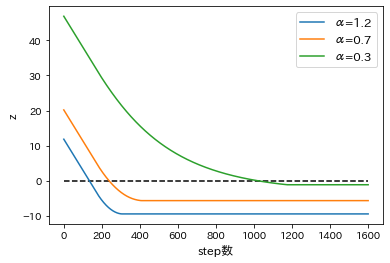
\includegraphics[scale=0.7]{/Users/shunsuke/Desktop/master-thesis/alpha11_25_2.png}
\caption{\eqref{z_method}において$\alpha=0.3,0.7,1.2$で比較した図}
\end{center}
\end{figure}

\begin{table}[h]
    %\caption{\eqref{z_method}において$\alpha=0.3,0.7,1.2$で比較した値}
    \label{table:colortbl}
    \centering
    \begin{tabular}{|r|r|r|}
     \hline
     $\alpha$ & オーバーシュート$[\mu m]$ & かかった時間$[ms]$  \\
     \hline\hline
     1.2 & 9.40 & 151 \\
     0.7 & 5.62 & 203 \\
     0.3 & 1.10 & 566\\
     \hline
    \end{tabular}
\end{table}
  
\eqref{table:colortbl}のように$\alpha$の値が小さくなるにつれ,オーバーシュートが小さくなるがプレスにかかる時間が長くなってしまう.


\begin{figure}[h]
    \begin{center}
    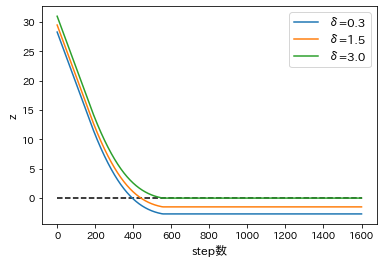
\includegraphics[scale=0.7]{/Users/shunsuke/Desktop/master-thesis/1129_delta.png}
    \caption{\eqref{z_method}において$\delta=0.3,1.5,3.0$で比較した図}
    \end{center}
\end{figure}

\begin{table}[h]
    %\caption{\eqref{z_method}において$\alpha=0.3,0.7,1.2$で比較した値}
    \label{table:colortbl2}
    \centering
    \begin{tabular}{|r|r|r|}
     \hline
     $\beta$ & オーバーシュート$[\mu m]$ & かかった時間$[ms]$  \\
     \hline\hline
     1.2 & 9.40 & 277 \\
     0.7 & 5.62 & 277 \\
     0.3 & 1.10 & 277 \\
     \hline
    \end{tabular}
\end{table}
\eqref{table:colortbl2}のように$\beta$の値が小さくなるにつれ,オーバーシュートは小さくなる.またかかった時間やプレスの速度は$\beta$に
依らないので変化しない.
\section{ばらつき}
\section{終章}
\subsection{結論}
\subsection{残された課題}
文献は\cite{Si}で表せます.
\begin{thebibliography}{9}
\bibitem{Si} A. Simoni\u{c}, The Ahlfors lemma and Picard's theorems, 
Rose-Hulman Undergrad. Math. J. {\bf 16} (2015), no. 2, 113--136. 
\bibitem{KF} 岸正倫,藤本坦孝,複素関数論,学術図書出版社 (1980).
\bibitem{Fu} 藤本坦孝,複素解析,岩波書店 (2006).


\end{thebibliography}

\end{document}
